\documentclass[12pt,a4paper]{scrreprt}
% KOMA script report style, font size 12pt, A4 size paper

\KOMAoptions{parskip=half,numbers=noenddot,listof=totoc,bibliography=totoc}
% Separate paragraphs with space, no end dot for section no.,
% list of figure and tables in TOC, biliography in TOC

\KOMAoptions{twoside=on,open=right}
% Two page printing, chapter opening on right page 

\def\chapmar{1}                         % 1=On, chap. no moved into margin

\usepackage{scrpage2}                   % Header and footer
\usepackage{mathpazo}                   % URW Palladio math font
\usepackage[no-math]{fontspec}          % Load custom otf font
\usepackage{polyglossia}                % Language support 
\usepackage{amsmath}                    % Math package				
\usepackage{graphicx}                   % Includegraphics
\usepackage[bf,up,hang]{subfigure}      % Subfigures
\usepackage[small,bf,up,hang]{caption}  % Better caption layout
\usepackage[percent]{overpic}           % Overlay symboles for graphs
\usepackage{nicefrac}                   % Diagonal fraction line
\usepackage{multirow}                   % Multirows for tables
\usepackage{booktabs}                   % Table rulers
\usepackage{colortbl}                   % Colored tables 
\usepackage{tabularx}                   % Adjutable table width
\usepackage{array}                      % Advanced table control
\usepackage{microtype}                  % Font expansion
\usepackage{xspace}                     % Enter space in macros
\usepackage{hyperref}                   % Hypertext reference
\usepackage{natbib}                     % Author-date system
\usepackage{listings}                   % Source code listing

% ---------------------------------------------------------------	
% Global Settings

% Syntax Highlighting
\lstset{%
	language=Matlab,
	basicstyle=\scriptsize\ttfamily,
	showstringspaces=false,
	tabsize=3,
	prebreak=\raisebox{0ex}[0ex][0ex]{\ensuremath{\hookleftarrow}},
	frame=single,
	keywordstyle=\color[rgb]{0,0,1},
	commentstyle=\color[rgb]{0.133,0.545,0.133},
	stringstyle=\color[rgb]{0.627,0.126,0.941},
	morekeywords={properties,methods,classdef},
	deletekeywords={eps,cond}}

% Figure Path
\graphicspath{{figures/}}

% Language Settings
\setdefaultlanguage{english}			
\setotherlanguage[spelling=new]{german}

% KOMA script options
\automark[subsection]{section}			
\clearscrheadfoot
\ohead[]{\headmark}
\ofoot[\pagemark]{\pagemark}

% Font Settings for Open Sans
\setsansfont[Ligatures=TeX,Numbers=OldStyle]{Open Sans}
\setmainfont[Ligatures=TeX,Numbers=Monospaced]{Palatino}
\setmonofont{Source Code Pro}
\newfontfamily\os{Open Sans}
\linespread{1.3}\selectfont

% Custom Commands
\newcommand{\HRule}{\rule{\linewidth}{1.4mm}}
\newcommand{\Matlab}{\href{http://www.mathworks.com}{MATLAB\textsuperscript{\tiny\textregistered} }}
\newcommand{\celsius}{{\rmfamily\textit{\textcelsius}}}
\newcommand\relphantom[1]{\mathrel{\phantom{#1}}}
\newcommand\cm[1]{\scalebox{1.6}[1.0]{\hspace{0.1mm}-\hspace{0.1mm}}{#1}}
%\newcolumntype{R}{>{\raggedleft\arraybackslash}X}


% PDF Setup
\hypersetup{%
pdfauthor={Alexander Zhou},
pdftitle={Thesis},
pdfcreator={pdfTeX},
pdfsubject={Lorem Ipsum},
pdfkeywords={Lorem ipsum},
colorlinks,citecolor=black,filecolor=black,linkcolor=black,urlcolor=black}

% ---------------------------------------------------------------
% Move numbers of section headings left into the margin

% Re-define \chapterformat only if it is defined and not
% \relax without making it \relax if it is not defined:

\ifthenelse{\chapmar=1}{
\begingroup
\expandafter\expandafter\expandafter\endgroup
\expandafter\ifx\csname chapterformat\endcsname\relax\else
  \renewcommand*{\chapterformat}{%
    \llap{%
      % Following line is the original definition
      \chapappifchapterprefix{\ }\thechapter\autodot\enskip
    }%
  }
\fi
 
% Re-define \othersectionlevelsformat
\renewcommand*{\othersectionlevelsformat}[1]{%
  \llap{%
    % Following line is the original definition
    \csname the#1\endcsname\autodot\enskip
  }%
}}

% ---------------------------------------------------------------
% Titlepage 

\begin{document}
	
% Enlarge this page, DIV=14, BCOR=14mm
\areaset[20mm]{165.0mm}{233.36mm}
\pagenumbering{roman}
\pagestyle{plain}
\thispagestyle{empty}
\begin{titlepage}\centering
  \begingroup
  \vspace*{\stretch{1}}
  {\os\huge\bfseries Title English\\[3mm]}
  \HRule\\
  {\huge\bfseries\textgerman{\os Title Deutsch}\\[6.0cm]}
  {\large Der \href{http://www.techfak.uni-erlangen.de/}{Technischen Fakult\"at} der\\\href{http://www.uni-erlangen.de/}{Universit\"at Erlangen-N\"urnberg}\\zur Erlangung des Grades\\[0.7cm]}
  {\os\large\bfseries DOKTOR INGENIEUR\\[0.7cm]}
  {\large vorgelegt von\\[0.5cm]}
  {\os\large\bfseries Diplom-Ingenieur Gaius Octavius\\[0.5cm]}
  {\large Erlangen 20xx\\}
  \endgroup
\end{titlepage}

% Reset the typing area, DIV=12, BCOR=14mm
\areaset[20mm]{157.5mm}{222.75mm}
\thispagestyle{empty}
\vspace*{\stretch{1}}
\begingroup
\begin{center}
Als Dissertation genehmigt von der\\[2mm]
Technischen Fakult\"at der Universit\"at Erlangen-N\"urnberg\\[1cm]
\end{center}
\begin{tabbing}
Tag der Einreichung: \= xx.xx.20xx\\[2mm]
Tag der Promotion:   \> xx.xx.20xx\\[2mm]
Dekanin:             \> Prof. Dr.-Ing. A\\[2mm]
Berichterstatter:    \> Prof. Dr.-Ing. B\\[2mm]
                     \> Prof. Dr.-Ing. C\\[2mm]
					 \> Prof. Dr.-Ing. D
\end{tabbing}
\endgroup
\pagebreak

% ---------------------------------------------------------------
% Abstract & Acknowledgement

%!TEX root = 00-Thesis-Main.tex
\chapter*{Danksagung}
\addcontentsline{toc}{chapter}{Danksagung}

Neque porro quisquam est qui dolorem ipsum quia dolor sit amet, consectetur, adipisci velit...	
%!TEX root = 00-Thesis-Main.tex
\chapter*{Zusammenfassung}

\begin{german}
Lorem ipsum dolor sit amet, consectetur adipiscing elit. Duis eu metus maximus, sodales nisi eu, accumsan dolor. Curabitur consectetur augue dui, vitae ultricies turpis rhoncus quis. Nulla laoreet libero ac ipsum euismod luctus. Nam vehicula dapibus libero, eget fermentum nibh. Nullam sagittis lorem id lobortis faucibus. Quisque varius, eros vitae pellentesque imperdiet, odio felis sodales mi, a euismod nulla urna vitae augue. Sed in nisl vel arcu dignissim vehicula at id urna. Class aptent taciti sociosqu ad litora torquent per conubia nostra, per inceptos himenaeos.
\end{german}
%!TEX root = 00-Thesis-Main.tex
\chapter*{Abstract}

Lorem Ipsum is simply dummy text of the printing and typesetting industry. Lorem Ipsum has been the industry's standard dummy text ever since the 1500s, when an unknown printer took a galley of type and scrambled it to make a type specimen book. It has survived not only five centuries, but also the leap into electronic typesetting, remaining essentially unchanged. It was popularised in the 1960s with the release of Letraset sheets containing Lorem Ipsum passages, and more recently with desktop publishing software like Aldus PageMaker including versions of Lorem Ipsum.

% ---------------------------------------------------------------
% Table of Contents

\tableofcontents
\listoffigures
%\pagebreak
\listoftables

% ---------------------------------------------------------------
% Document

%!TEX root = 00-Thesis-Main.tex
\chapter*{Nomenclature}
\addcontentsline{toc}{chapter}{Nomenclature}

\section*{Latin Letters}
\begin{tabbing}
$\quad$\=$Syb$\hspace{2.45cm}\=some text\hspace{7.5cm}\=$big unit/big unit$\=end\kill
\>$E$\>Energy\>$J$\\
\>$m$\>Mass\>$kg$\\
\>$c$\>Speed of light\>$km/s$\\
\end{tabbing}



\pagestyle{scrheadings}
\pagenumbering{arabic}
\setcounter{page}{1}
\bibliographystyle{alpha}

\part*{T H E S I S}
\setcounter{chapter}{-1}
%!TEX root = 00-Thesis-Main.tex
\chapter{Einleitung}

\begin{german}
Lorem Ipsum ist ein einfacher Demo-Text für die Print- und Schriftindustrie. Lorem Ipsum ist in der Industrie bereits der Standard Demo-Text seit 1500, als ein unbekannter Schriftsteller eine Hand voll Wörter nahm und diese durcheinander warf um ein Musterbuch zu erstellen. Es hat nicht nur 5 Jahrhunderte überlebt, sondern auch in Spruch in die elektronische Schriftbearbeitung geschafft (bemerke, nahezu unverändert). Bekannt wurde es 1960, mit dem erscheinen von "Letraset", welches Passagen von Lorem Ipsum enhielt, so wie Desktop Software wie "Aldus PageMaker" - ebenfalls mit Lorem Ipsum.
\end{german}
%!TEX root = 00-Thesis-Main.tex
\chapter{Introduction}

Lorem ipsum dolor sit amet, consectetur adipiscing elit. Duis eu metus maximus, sodales nisi eu, accumsan dolor. Curabitur consectetur augue dui, vitae ultricies turpis rhoncus quis. Nulla laoreet libero ac ipsum euismod luctus. Nam vehicula dapibus libero, eget fermentum nibh. Nullam sagittis lorem id lobortis faucibus. Quisque varius, eros vitae pellentesque imperdiet, odio felis sodales mi, a euismod nulla urna vitae augue. Sed in nisl vel arcu dignissim vehicula at id urna. Class aptent taciti sociosqu ad litora torquent per conubia nostra, per inceptos himenaeos.

Etiam blandit neque feugiat, efficitur ante in, euismod urna. Donec laoreet, nisl vitae placerat dictum, ipsum velit hendrerit lectus, sit amet mollis elit ligula a libero. Cras ut imperdiet mi. Ut quis ultricies sapien. Suspendisse vel vehicula est, nec semper arcu. Nullam tincidunt sagittis magna nec ultricies. Sed gravida purus id nisi vehicula, sit amet gravida enim mattis. Class aptent taciti sociosqu ad litora torquent per conubia nostra, per inceptos himenaeos. Pellentesque sollicitudin metus ac commodo viverra. Morbi ultrices mattis lobortis. Donec libero sapien, scelerisque id pulvinar et, aliquet tempus dolor. Curabitur leo risus, venenatis a dapibus a, convallis quis magna.
%!TEX root = 00-Thesis-Main.tex
\chapter{Faber Est Quisque Fortunae Suae}\label{cha:fortune}

Lorem ipsum dolor sit amet, consectetur adipiscing elit. Duis eu metus maximus, sodales nisi eu, accumsan dolor. Curabitur consectetur augue dui, vitae ultricies turpis rhoncus quis. Nulla laoreet libero ac ipsum euismod luctus. Nam vehicula dapibus libero, eget fermentum nibh. Nullam sagittis lorem id lobortis faucibus. Quisque varius, eros vitae pellentesque imperdiet, odio felis sodales mi, a euismod nulla urna vitae augue. Sed in nisl vel arcu dignissim vehicula at id urna. Class aptent taciti sociosqu ad litora torquent per conubia nostra, per inceptos himenaeos.

\begin{equation}
	E=mc^2\label{eq:Einstein}.
\end{equation}

Etiam blandit neque feugiat, efficitur ante in, euismod urna. Donec laoreet, nisl vitae placerat dictum, ipsum velit hendrerit lectus, sit amet mollis elit ligula a libero. Cras ut imperdiet mi. Ut quis ultricies sapien. Suspendisse vel vehicula est, nec semper arcu. Nullam tincidunt sagittis magna nec ultricies. Sed gravida purus id nisi vehicula, sit amet gravida enim mattis. Class aptent taciti sociosqu ad litora torquent per conubia nostra, per inceptos himenaeos. Pellentesque sollicitudin metus ac commodo viverra. Morbi ultrices mattis lobortis. Donec libero sapien, scelerisque id pulvinar et, aliquet tempus dolor. Curabitur leo risus, venenatis a dapibus a, convallis quis magna.
%!TEX root = 00-Thesis-Main.tex
\chapter{Aut Vincere Aut Mori}\label{cha:conquer}

Lorem ipsum dolor sit amet, consectetur adipiscing elit. Duis eu metus maximus, sodales nisi eu, accumsan dolor. Curabitur consectetur augue dui, vitae ultricies turpis rhoncus quis. Nulla laoreet libero ac ipsum euismod luctus. Nam vehicula dapibus libero, eget fermentum nibh. Nullam sagittis lorem id lobortis faucibus. Quisque varius, eros vitae pellentesque imperdiet, odio felis sodales mi, a euismod nulla urna vitae augue. Sed in nisl vel arcu dignissim vehicula at id urna. Class aptent taciti sociosqu ad litora torquent per conubia nostra, per inceptos himenaeos.


\begin{figure}[ht!]\centering
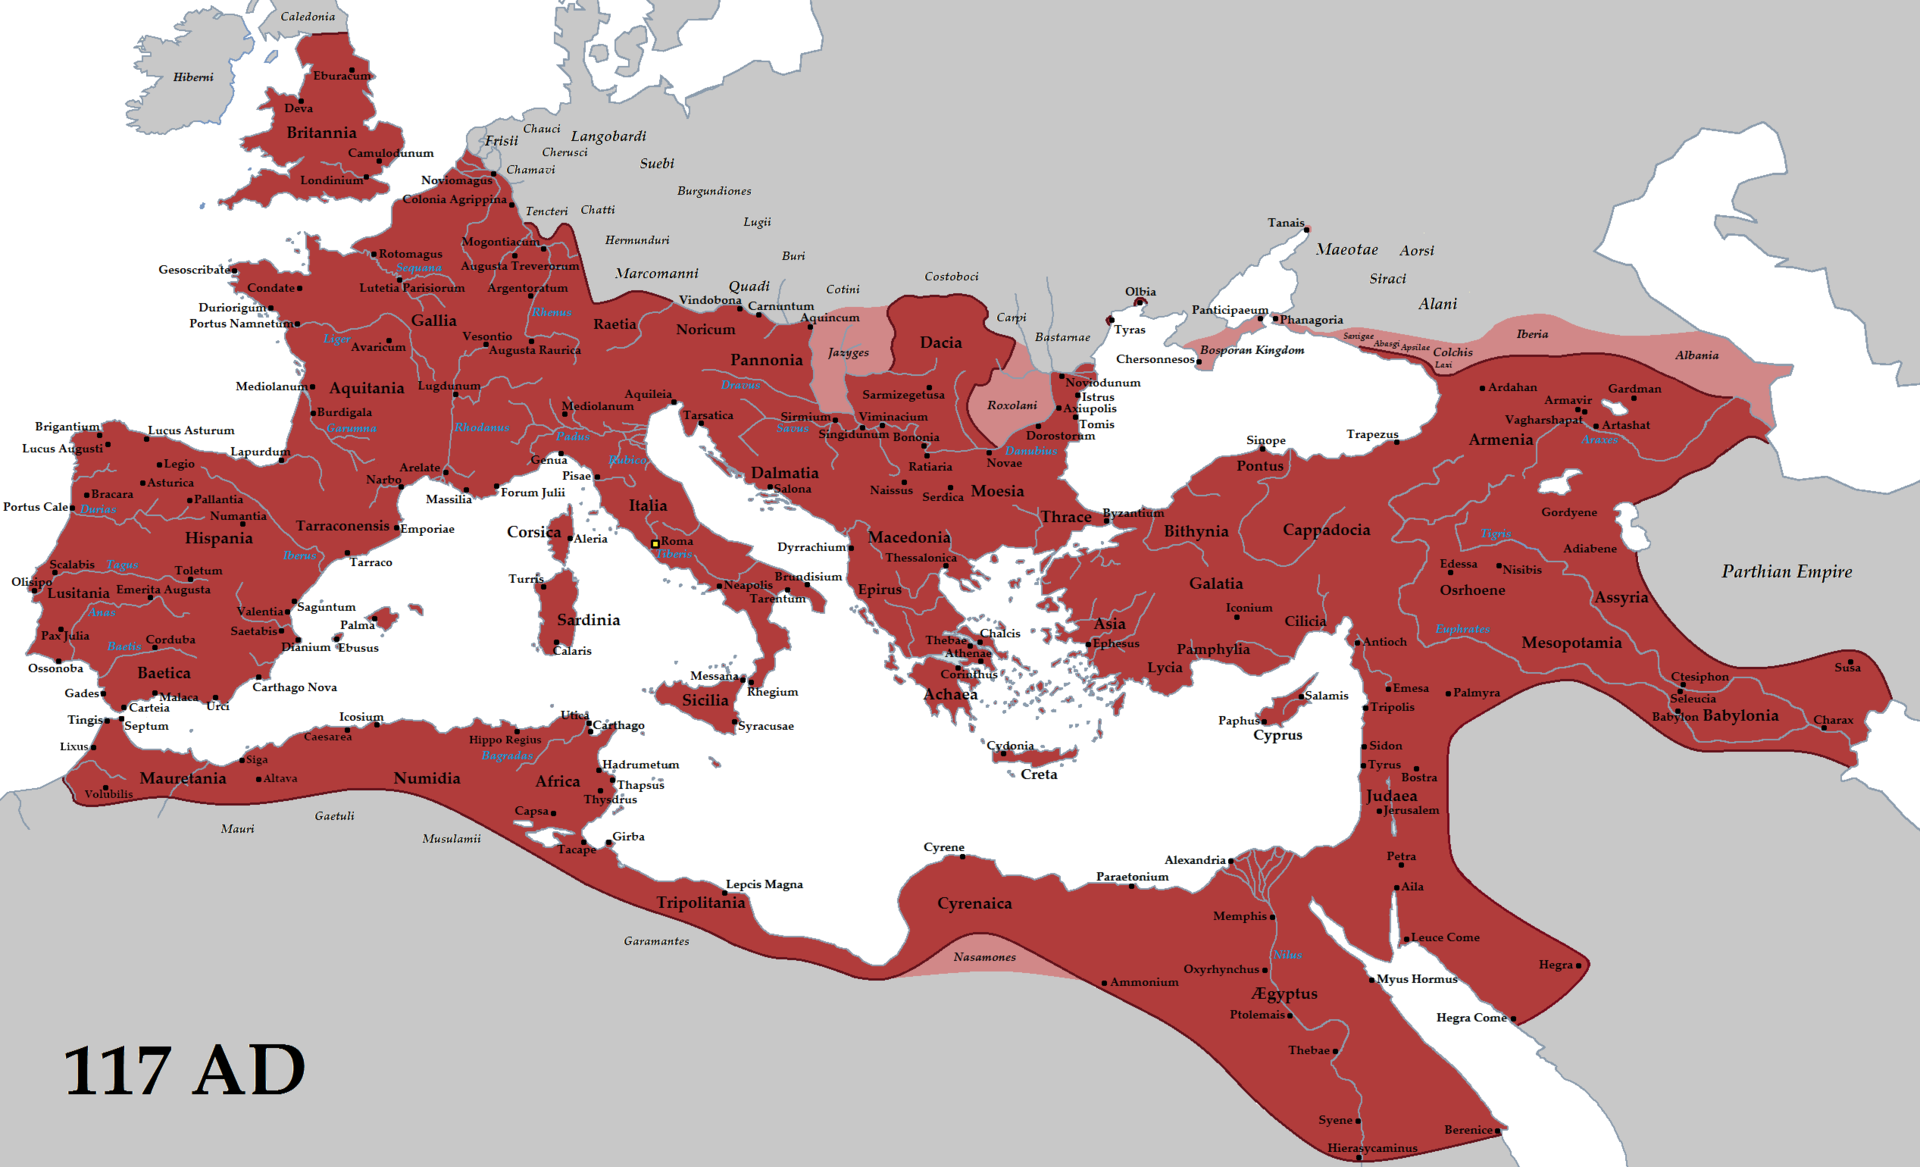
\includegraphics[width=0.8\linewidth]{romanEmpireTrajan}
\caption{The Roman Empire in 117 AD, at its greatest exten, Source: Wikipedia\label{fig:romanEmpireTrajan}}
\end{figure}

Etiam blandit neque feugiat, efficitur ante in, euismod urna. Donec laoreet, nisl vitae placerat dictum, ipsum velit hendrerit lectus, sit amet mollis elit ligula a libero. Cras ut imperdiet mi. Ut quis ultricies sapien. Suspendisse vel vehicula est, nec semper arcu. Nullam tincidunt sagittis magna nec ultricies. Sed gravida purus id nisi vehicula, sit amet gravida enim mattis. Class aptent taciti sociosqu ad litora torquent per conubia nostra, per inceptos himenaeos. Pellentesque sollicitudin metus ac commodo viverra. Morbi ultrices mattis lobortis. Donec libero sapien, scelerisque id pulvinar et, aliquet tempus dolor. Curabitur leo risus, venenatis a dapibus a, convallis quis magna.

\begin{table}[ht!]\centering\small{\addfontfeatures{Numbers={Monospaced}}
\begin{tabularx}{0.4\textwidth}{Xrr}
\toprule
Province & Tax & Citizen\\
\midrule
\rowcolor[gray]{0.9}Arabia      & 1 & 2 \\
					Palaestina  & 3 & 4 \\ 
\rowcolor[gray]{0.9}Syria	    & 5 & 6 \\
					Phoenice    & 7 & 8 \\ 
\bottomrule     	
\end{tabularx}}
\caption{Roman Provinces\label{tab:romanProvinces}}
\end{table}

Ut sapien lacus, mollis porttitor convallis a, dignissim rhoncus dolor. Ut sit amet placerat enim, eu ornare turpis. Duis ante tellus, molestie sit amet urna a, lobortis pharetra sem. Nullam faucibus urna purus, at congue justo molestie a. Pellentesque lobortis velit turpis. Etiam sit amet augue faucibus, laoreet orci eu, lobortis metus. Phasellus vulputate, turpis a blandit aliquet, justo ex sollicitudin turpis, eget vestibulum sem augue nec enim. Phasellus a sem vel metus pulvinar consectetur. In ultricies magna at sem rhoncus hendrerit. Integer eget elementum velit. Sed consequat laoreet erat sit amet porttitor.

Suspendisse lobortis aliquam tortor quis aliquam. Vestibulum et nisi at justo tincidunt rutrum. Nullam in magna odio. Aliquam velit urna, ultrices sit amet faucibus eu, molestie eu urna. In hac habitasse platea dictumst. Proin blandit aliquam commodo. Cras nec ullamcorper risus.

Sed eleifend dictum lorem, in luctus neque efficitur a. Etiam fringilla non mi condimentum tempus. Etiam scelerisque sem sit amet arcu egestas consequat. Aenean ut nibh ut quam ullamcorper pretium. Pellentesque vitae malesuada urna. Aliquam mauris ante, tincidunt sit amet lacinia tempor, congue ac enim. Maecenas vitae leo efficitur, maximus dui vel, ultricies dui. Praesent egestas lorem est, sed finibus lorem consequat at. Ut rhoncus risus accumsan libero ornare, ut lacinia metus cursus. Cum sociis natoque penatibus et magnis dis parturient montes, nascetur ridiculus mus. Aliquam lacinia molestie rutrum. Donec quis dictum elit. Nulla facilisi. Praesent at pulvinar tortor, vel interdum sem. Quisque maximus semper urna in mattis.

\pagestyle{scrplain}
%!TEX root = 00-Thesis-Main.tex
\chapter{Conclusion}\label{cha:conclusion}

Lorem ipsum dolor sit amet, consectetur adipiscing elit. Duis eu metus maximus, sodales nisi eu, accumsan dolor. Curabitur consectetur augue dui, vitae ultricies turpis rhoncus quis. Nulla laoreet libero ac ipsum euismod luctus. Nam vehicula dapibus libero, eget fermentum nibh. Nullam sagittis lorem id lobortis faucibus. Quisque varius, eros vitae pellentesque imperdiet, odio felis sodales mi, a euismod nulla urna vitae augue. Sed in nisl vel arcu dignissim vehicula at id urna. Class aptent taciti sociosqu ad litora torquent per conubia nostra, per inceptos himenaeos.

Etiam blandit neque feugiat, efficitur ante in, euismod urna. Donec laoreet, nisl vitae placerat dictum, ipsum velit hendrerit lectus, sit amet mollis elit ligula a libero. Cras ut imperdiet mi. Ut quis ultricies sapien. Suspendisse vel vehicula est, nec semper arcu. Nullam tincidunt sagittis magna nec ultricies. Sed gravida purus id nisi vehicula, sit amet gravida enim mattis. Class aptent taciti sociosqu ad litora torquent per conubia nostra, per inceptos himenaeos. Pellentesque sollicitudin metus ac commodo viverra. Morbi ultrices mattis lobortis. Donec libero sapien, scelerisque id pulvinar et, aliquet tempus dolor. Curabitur leo risus, venenatis a dapibus a, convallis quis magna.


\part*{A P P E N D I X}
\appendix
%!TEX root = 00-Thesis-Main.tex
\chapter{Quotes}
\section{Divide}\label{app:divice}
Divide et impera 

\section{KOMA-Script}\label{app:koma}
The KOMA-Script \cite{kohm93} bun­dle pro­vides re­place­ments for the ar­ti­cle, re­port, and book classes with em­pha­sis on ty­pog­ra­phy and ver­sa­til­ity. 
\bibliography{references/Sample}{}

\end{document}

